\chapter{Experiments}


\begin{figure}[!hbt]
  \centering
  \input{tirf-exp.eps_tex} 
  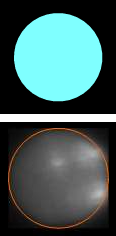
\includegraphics[height=60.48mm]{screen_mma-disk-integrate_rot}
  \caption{A fluorescent plane on a slide is embedded in oil, water or
    air. The thickness of the embedding medium is approximately
    $\unit[5]{\mu m}$. The LCoS illuminates a disk with $\unit[30]{\mu
      m}$ diameter while a $15\times 15$ window is scanned over the
% 200 px diameter on LCoS
    MMA. {\bf right top:} LCoS mask. {\bf right bottom:} Typical
    camera image.}
  \label{fig:tirf-exp}
\end{figure}


\begin{figure}[!hbt]
  \centering
  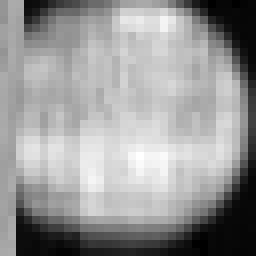
\includegraphics[width=4cm]{oil}
  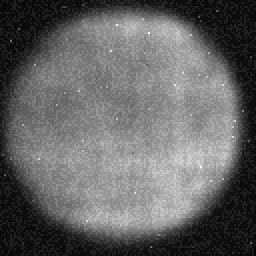
\includegraphics[width=4cm]{water}
  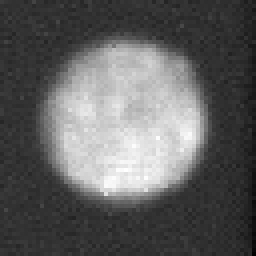
\includegraphics[width=4cm]{air}
  \caption{dfaxs}
  \label{fig:immersion-bfp-scan}
\end{figure}
